% =====================================================================
\section{실패 분석}
\label{sec:failure}
% =====================================================================

본 절은 Regime Map에서 관찰되는 우위 역전이 \emph{왜} 일어나는지에 대한 메커니즘 수준의 증거를 제시한다.

\subsection{Baseline--overlap--기하 불확실도의 관계}
\label{sec:confound}

두 view로 3D 점을 삼각측량하는 문제는 재투영 오차를 최소화하는 비선형 최소제곱이며, Gauss--Newton 근사 아래에서 추정치의 공분산은 다음과 같이 주어진다~\cite{hartley2003multiple}.
\begin{equation}
\mathrm{Cov}(\hat\beta) \;\approx\; \sigma^2 \bigl(J^\top J\bigr)^{-1}
\label{eq:covariance}
\end{equation}
여기서 $J = \partial r / \partial \beta$는 재투영 오차의 야코비안이고 $\sigma$는 관측 노이즈의 표준편차다. 정렬된 두 view의 단순한 경우 식~\eqref{eq:covariance}의 깊이 성분은 $\sigma_Z \propto Z^2/(fB)$로 정리되며($f$는 초점거리, $B$는 baseline, $Z$는 깊이), 가로 방향 불확실도와의 비는 $\sigma_Z/\sigma_X \propto Z/B$가 된다.

즉 지배 변수는 baseline 자체가 아니라 \textbf{시차비 $B/Z$}이다. 이는 baseline과 overlap이 서로 다른 개념임을 함의한다. Baseline을 키우면 삼각측량 정밀도는 개선되지만 시점 차이가 커져 대응점 탐색이 어려워지고 co-visibility는 감소하므로, 두 요인은 반대 방향으로 작용한다.

이 관계를 실제 데이터에서 진단적으로 검증하였다. DTU scan1의 42-view 재구성에서 모든 view pair(861쌍)에 대해 baseline(카메라 중심 간 거리), overlap(식~\eqref{eq:overlap}), 식~\eqref{eq:covariance} 기반 깊이 불확실도를 계산한 결과, 원시 상관은 $\mathrm{corr}(O_{ij},\ \log\hat\sigma_{\mathrm{depth}}) = +0.952$로 ``overlap이 높을수록 불확실도가 낮다''는 예상과 반대 부호를 보였다.

Baseline을 \emph{선형으로} 통제한 편상관은 $+0.801$로 소폭만 감소했으나, baseline과 불확실도의 관계가 선형이 아니라 거듭제곱 형태임을 확인한 뒤($\mathrm{corr}(\log B,\ \log\hat\sigma) = -0.989$, 선형 버전 $-0.951$) $\log B$로 통제하자 편상관이 $+0.301$로 크게 감소했다.

이 결과의 해석은 두 가지다. 첫째, 부호 역전 자체는 위의 이론과 정합적이다. DTU와 같은 궤도형(orbital) 촬영에서는 두 카메라가 가까울수록 overlap이 크고 동시에 baseline이 작으므로, overlap과 깊이 불확실도가 함께 증가하는 것이 기하학적으로 예측되는 결과다. 둘째, $\log B$ 통제 후에도 잔여 상관 $+0.301$이 남는다는 점은 overlap이 baseline으로 완전히 환원되지는 않음을 시사한다. 따라서 본 연구는 overlap을 주 축으로 유지하되, ``왜 저겹침 조건이 어려운가''에 대한 \emph{설명}은 overlap 자체가 아니라 그 배후의 baseline/parallax 기하에 귀속시킨다.

\begin{figure*}[t]
\centering
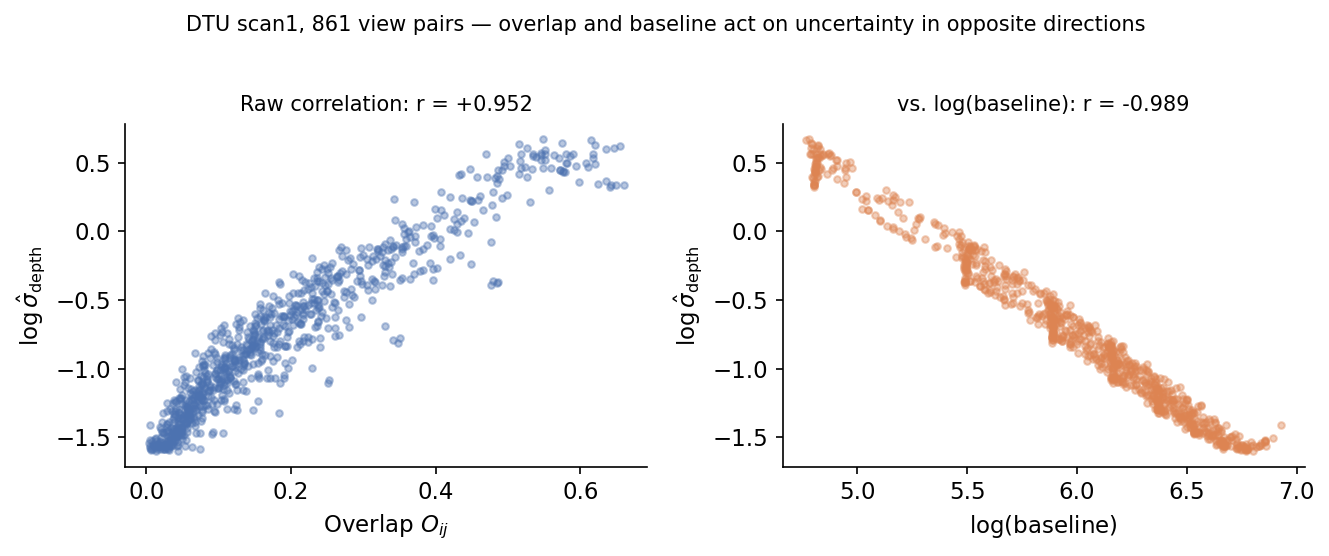
\includegraphics[width=0.8\linewidth]{figures/geometry_confound.png}
\caption{Overlap과 $\log(\mathrm{baseline})$이 깊이 불확실도($\log\hat\sigma_{\mathrm{depth}}$)와 맺는 관계. 왼쪽: 원시 overlap--불확실도 상관은 예상과 반대 부호($r=+0.952$). 오른쪽: $\log(\mathrm{baseline})$과의 관계는 거의 완벽한 선형($r=-0.989$) — baseline 교란이 부호 역전의 주 원인임을 시사한다. DTU scan1, 861 view pair.}
\label{fig:confound}
\end{figure*}

\chk{DTU는 궤도형 rig이므로 overlap과 baseline이 강하게 결합되어 있다. RE10K/DL3DV처럼 경로형(trajectory) 촬영에서는 두 변수의 결합 강도가 다를 수 있으므로 동일 분석을 반드시 반복할 것}

\subsection{Densification gradient의 관측 부족}
\label{sec:starvation}

gsplat~\cite{ye2024gsplat}의 기본 densification 전략은 매 100-iteration window마다 각 Gaussian의 2D 위치 gradient norm 평균을 고정 임계값 $\tau_{\mathrm{pos}} = 2\times 10^{-4}$와 비교해 성장 여부를 결정한다. 이 판단은 $\mathrm{grad2d}[g]\,/\,\mathrm{count}[g]$로 계산되며, $\mathrm{count}[g]$는 해당 Gaussian이 그 window 동안 관측된 횟수(effective observation count)다.

원래 가설은 ``관측이 적은 Gaussian일수록 평균 추정이 노이즈에 취약해 densification을 잘못 유발한다''는 것이었으나, 실측 결과 $\mathrm{count}[g] \le 2$인 Gaussian이 임계값을 초과하는 비율은 모든 조건에서 사실상 0\%(0.00--0.003\%)로 이 가설은 기각되었다. 관측이 적으면 분자인 누적 gradient도 함께 작아지기 때문이다.

대신 \textbf{관측 부족 Gaussian의 비율 자체가 view 수에 강하게 좌우된다}는 것을 발견했다(그림~\ref{fig:starvation}, 표~\ref{tab:starvation}). RE10K 3-scene, 2000-iteration 계측에서 $\mathrm{count}[g] \le 2$인 Gaussian의 비율은 2-view에서 51.5\%, 4-view에서 30.8\%, 8-view에서 3.2\%, 12-view에서 0.7\%로 단조 감소했다. 초기화 방식(COLMAP triangulation 성공 여부에 따른 sparse init 대 random-sphere fallback)이라는 교란요인을 제거하기 위해 4개 view 수 조건 모두 동일하게 random-sphere fallback을 사용한 단일 scene을 별도로 확인한 결과에서도 55.3\% $\to$ 32.3\% $\to$ 8.3\% $\to$ 1.3\%로 같은 패턴이 재현되어, 이 효과가 초기화 방식이 아니라 view 수 자체에 기인함을 확인했다.

\begin{figure}[t]
\centering
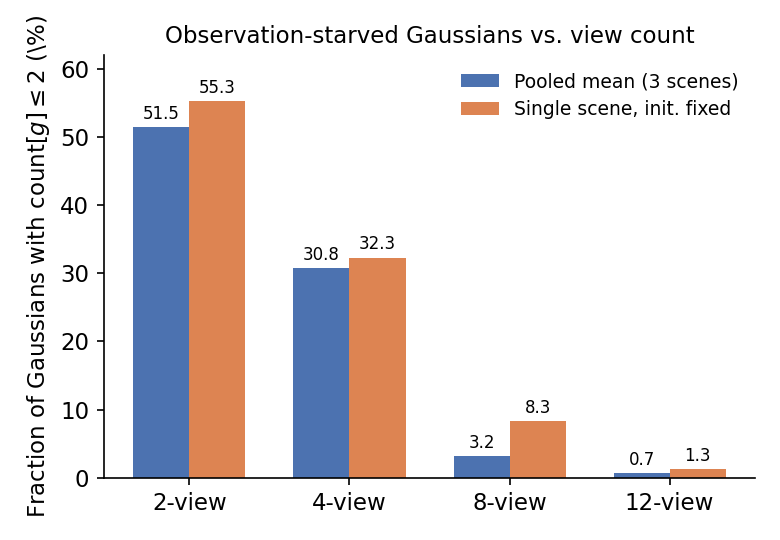
\includegraphics[width=0.95\linewidth]{figures/observation_starvation.png}
\caption{$\mathrm{count}[g] \le 2$인(=최근 100-iteration window에서 2번 이하로만 관측된) Gaussian의 비율. View 수가 늘수록 급격히 감소하며, 초기화 방식(sparse COLMAP init 대 random-sphere fallback)을 고정한 단일 scene에서도 동일한 패턴이 재현된다.}
\label{fig:starvation}
\end{figure}

\begin{table}[h]
\centering
\caption{관측 부족 Gaussian($\mathrm{count}[g] \le 2$)의 비율. RE10K 3-scene, 2000 iteration, seed 0}
\label{tab:starvation}
\small
\begin{tabular}{@{}l cccc@{}}
\toprule
조건 & 2-view & 4-view & 8-view & 12-view \\
\midrule
Pooled 평균 & 51.5\% & 30.8\% & 3.2\% & 0.7\% \\
초기화 고정(단일) & 55.3\% & 32.3\% & 8.3\% & 1.3\% \\
\bottomrule
\end{tabular}
\end{table}

이는 sparse-view에서 optimization이 불리한 이유를 ``데이터가 적다''는 추상적 설명을 넘어, \textbf{Gaussian 예산의 상당 부분이 어떤 학습 구간에서도 유의미한 gradient 신호를 받지 못한 채 방치된다}는 구현 수준에서 추적 가능한 메커니즘으로 제시한다. 이 Gaussian들은 gradient 신호가 미약하여 gradient 기반 densification의 대상이 되지도 못하고, 그렇다고 임계값을 넘어 잘못된 성장을 유발하지도 않으며, 사실상 사용되지 않는 모델 용량으로 남는다.

\chk{현재 결과는 두 원인이 섞여 있을 수 있다. (i) 관측 부족: Gaussian은 적절히 배치되었으나 카메라 수가 적어 소수 view에서만 보이는 경우, (ii) 배치 실패: random-sphere fallback으로 뿌린 점이 애초에 어떤 카메라 절두체에도 포함되지 않는 경우. 어떤 view에도 투영되지 않는 Gaussian의 비율을 별도로 측정해 (ii)를 분리해야 하며, 그 결과에 따라 본 절의 주장이 ``sparse-view 일반의 메커니즘''인지 ``triangulation 실패 시 random 초기화의 한계''인지가 갈린다}

\paragraph{사후 발견으로서의 위치} 본 절의 관측은 사전 등록한 가설 H1--H3에 포함되지 않았던 탐색적 발견(exploratory finding)이다. 따라서 확증적 결과와 구분하여 서술하며, 주 데이터셋 전체 규모에서의 재현 여부를 별도로 보고한다.

\subsection{사전 등록 가설의 검증}
\label{sec:h2-verification}

\begin{table*}[t]
\centering
\caption{사전 등록 가설과 검증 상태}
\label{tab:hypotheses}
\small
\begin{tabular}{@{}l L{12cm} L{2.6cm}@{}}
\toprule
가설 & 내용 & 상태 \\
\midrule
H1 & 초기 geometry 오차($\sigma$)가 커질수록 densification 이후 Gaussian 수는 증가하지만 held-out 품질은 감소하며, 이 관계는 저겹침 조건에서 강화된다 & 절반 지지, 절반 기각(\S\ref{sec:c2}) \\
H2 & Optimization의 품질 정점 도달 시점은 view 수가 줄수록 앞당겨지고, 정점 이후 하강 기울기가 가팔라진다 & 부분 지지 (아래) \\
H3 & 초기 geometry 품질이 일정 수준을 넘으면 refinement의 한계 이득이 소멸한다 & 잠정 지지, 교란 미분리 (\S\ref{sec:c1b}) \\
\bottomrule
\end{tabular}
\end{table*}

세 가설 중 어느 것이 기각되더라도 그 자체가 보고 대상이다. 실제로 \S\ref{sec:starvation}에서 원래 가설(관측 부족으로 인한 오탐)이 기각되고 다른 메커니즘(관측 부족 자체의 비율)이 발견된 사례가 있었다.

\paragraph{H2 검증} RE10K C1-a 궤적 로그(scene당 예산 스냅샷 4개: 1/10/60/300\,s)에서, 4개 지점 중 test PSNR 최댓값이 300\,s 이전(=``조기 정점'')에 나타나는 비율을 view 수별로 집계했다.

\textbf{정점 시점 부분은 지지된다}: 조기 정점 비율은 Vanilla3DGS에서 2-view 91.7\% $\to$ 12-view 63.3\%, FSGS에서 2-view 91.7\% $\to$ 12-view 18.3\%로 두 방법 모두 view 수가 늘수록 단조 감소했다 — view가 적을수록 정점이 일찍 온다는 예측과 일치한다.

그러나 \textbf{하강 기울기 부분은 기각된다}: 조기 정점 발생 시 정점 대비 300\,s 하강폭(scene cluster bootstrap 95\% CI)은 Vanilla3DGS에서 오히려 view 수가 늘수록 커졌다(2-view $0.69\,$dB $[0.45,0.95]$ $\to$ 12-view $2.80\,$dB $[1.88,3.93]$) — 예측과 정반대 방향이다. FSGS에서는 뚜렷한 추세 없이 $0.5$--$0.9\,$dB 범위에 머물렀다(단 12-view는 조기 정점 표본이 scene 7개뿐이라 CI가 넓음).

정점 시점이 앞당겨지는 것과 하강이 가팔라지는 것은 별개 현상이며, 후자는 view 수 자체보다 densification/opacity reset 주기와 예산 경계의 상호작용에 더 좌우되는 것으로 보인다 — 이는 \S\ref{sec:results}에서 관찰한 12-view Vanilla3DGS의 비단조성과 같은 계열의 현상일 가능성이 있다.

\chk{\textbf{표본 해상도의 한계}: 예산 스냅샷이 1/10/60/300\,s 4개뿐이라 ``정점 시점''과 ``하강 기울기'' 추정 모두 해상도가 매우 거칠다 — 실제 정점이 이 4개 지점 \emph{사이}에 있어도 가장 가까운 스냅샷으로만 근사된다. 특히 위 하강폭 결과(view 수가 늘수록 하강이 커짐)는 12-view Vanilla3DGS의 60\,s 지점 비단조성(\S\ref{sec:results}) 자체가 4점 표본에 어떻게 걸리느냐에 따라 만들어졌을 수 있다 — 이 조악한 표본으로는 ``하강이 실제로 view 수에 따라 커진다''와 ``60\,s 근방의 일시적 하락이 우연히 하강폭으로 잡혔다''를 구분할 수 없다. 더 촘촘한 예산 스냅샷(예: 5/15/30/60/120/300\,s)으로 재실행해야 이 둘을 가른다.}

\subsection{Depth 불확실도 개입}
\label{sec:c2}

DTU 8-scan 외부 검증에서 두 종류의 통제된 depth 왜곡을 대표 조건 4개(\texttt{2view\_low\_overlap}, \texttt{4view\_low\_overlap}, \texttt{4view\_high\_overlap}, \texttt{12view\_high\_overlap}) $\times$ seed\{0,1\}에 주입했다: (a) 개별 노이즈 $d' = d(1+\varepsilon)$, $\varepsilon \sim \mathcal{N}(0,\sigma^2)$, $\sigma \in \{0, 0.01, 0.03, 0.05, 0.10\}$, (b) 전역 스케일 편향 $d' = s \cdot d$, $s \in \{0.9, 0.95, 1.0, 1.05, 1.1\}$(단안·저겹침 조건의 절대 스케일 미결정성~\cite{hartley2003multiple}을 모사). 640 combo 전량(2560 rows) 완주했다. 아래는 budget=300\,s 시점, scene cluster bootstrap 기준.

\begin{figure*}[t]
\centering
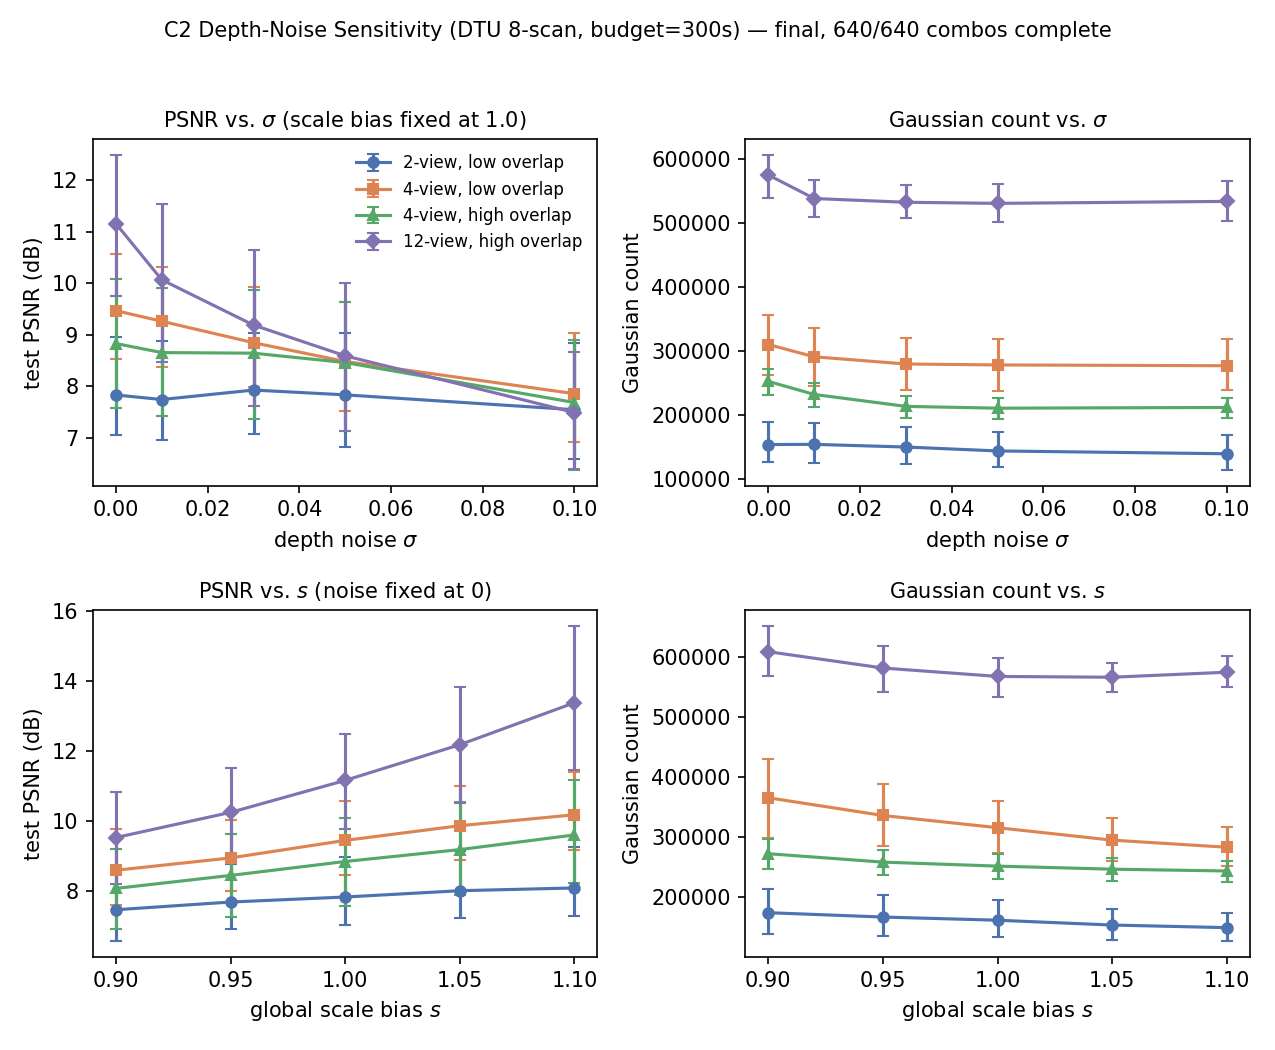
\includegraphics[width=0.85\linewidth]{figures/c2_depth_sensitivity.png}
\caption{C2 depth-noise sensitivity, DTU 8-scan, budget=300\,s. 위 행은 개별 노이즈 $\sigma$ 축, 아래 행은 전역 스케일 편향 $s$ 축. 왼쪽 열(PSNR)은 4개 조건 모두 예측대로 하락(위)/비대칭 단조 증가(아래)하지만, 오른쪽 열(Gaussian 수)은 H1이 예측한 증가가 아니라 하락 또는 평탄이다. 오차 막대는 scene cluster bootstrap 95\% CI.}
\label{fig:c2-sensitivity}
\end{figure*}

\begin{table}[h]
\centering
\caption{H1 예측 대 결과 요약(C2, DTU 8-scan).}
\label{tab:h1-summary}
\small
\begin{tabular}{@{}L{3.3cm} L{3.6cm}@{}}
\toprule
예측 & 결과 \\
\midrule
$\sigma$ $\uparrow$ $\Rightarrow$ PSNR $\downarrow$ & 지지(4개 조건 전부, $r=-0.06$~$-0.51$) \\
$\sigma$ $\uparrow$ $\Rightarrow$ Gaussian 수 $\uparrow$ & 기각 — 반대(4개 조건 전부 하락/평탄, $r=-0.13$~$-0.38$) \\
저겹침에서 두 경향 강화 & 부분 지지($\sigma$축만, 유일 비교쌍인 4-view에서 근소) \\
\bottomrule
\end{tabular}
\end{table}

\paragraph{$\sigma$(개별 노이즈) 축} PSNR은 4개 조건 전부에서 $\sigma$가 커질수록 하락했다(예: 12-view 고겹침 $11.15 \to 7.49\,$dB, $r=-0.51$) — H1의 첫 절반은 지지된다. 그러나 \textbf{Gaussian 수는 4개 조건 전부에서 하락 또는 평탄}했다(예: 12-view 고겹침 $575{,}642 \to 534{,}311$, $r=-0.20$) — ``densification이 나쁜 geometry를 더 많은 Gaussian으로 보정하려 한다''는 두 번째 절반과 정반대다. 노이즈가 gradient 신호 자체를 훼손해 \S\ref{sec:starvation}의 \texttt{count[g]}가 임계값을 덜 넘기게 되고, 그 결과 densification이 오히려 억제되는 것으로 보인다 — \S\ref{sec:starvation}에서 발견한 관측-count 메커니즘과 같은 축의 설명이다.

\paragraph{$s$(전역 스케일 편향) 축} $s=1.0$을 중심으로 대칭적인 U자(0.9와 1.1이 비슷하게 나쁘고 1.0이 최고)를 사전에 기대했으나, 실제로는 \textbf{4개 조건 전부에서 $s=0.9\to1.1$까지 PSNR이 단조 증가}했다(예: 12-view 고겹침 $9.52\to13.37\,$dB) — 탐색 범위 안에서 정점을 찾지 못했다. $s=1.05$/$1.1$이 ``정답 스케일''인 $s=1.0$보다 항상 낫다는 것은, 본 연구의 depth 추정 파이프라인 자체에 계통적 과소추정 편향이 있어 $s>1.0$이 그 편향을 부분 상쇄하고 있을 가능성을 시사한다. 왜곡된 스케일이 ``진짜로 더 좋다''는 결론이 아니라, 탐색 범위를 벗어난 곳에 정점이 있을 가능성을 배제하지 못한다는 뜻으로 해석한다.

\paragraph{Overlap 증폭 효과} 같은 view 수에서 overlap만 다른 직접 비교쌍은 4-view 하나뿐이다(2-view는 저겹침만, 12-view는 고겹침만 설계에 있음). $\sigma$축은 저겹침이 근소하게 더 가파르게 하락했으나($-1.61\,$dB 대 $-1.14\,$dB), $s$축은 사실상 차이가 없었다($+1.59\,$dB 대 $+1.53\,$dB) — H1의 저겹침 증폭 예측은 절반의 절반만 지지된다.

\chk{자세한 조건별 수치와 재현 커맨드는 findings 폴더의 2026-08-19자 C2 분석 문서 참고. $s$축 탐색 범위 확장($s \in \{1.15, 1.2, 1.3\}$)과 Gaussian growth/prune 카운트 분리 계측이 다음 단계로 남아 있다.}
